\section{Standard Bangla license plate}
\subsection{Vehicle types}
Vehicles are of different types in Bangladesh. As a result license plates don't stay at the same place for each vehicle.
Vehicles considered in this thesis work are - private car, bus, cng auto-rickshaw, truck. Though there were no previous format and standardization of the license plate in the past, currently government has enforced digital license plate for all vehicles which makes it a new case to handle and less error prone than the previous systems.

\subsection{Structure of the plate}
The digital Bengali license plate is normally written in two lines.

    \begin{figure}[ht]
    \centering
    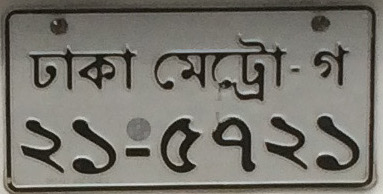
\includegraphics[scale=0.8]{./img/sample_plate}
    \caption{Example of a digital license plate in Bangla}
	\label{fig:EX}
    \end{figure}

\par
As the example given the line on the top written in Bangla and the bottom line has all digits in Bangla.    

\subsection{Parts of plate number}
The top line got two parts. First part before the '-' denotes the city of the car license and then the second part denotes the series it is in.

The bottom line is the number of the license assigned to the particular vehicle by the licensing rules and regulation of Bangladesh Road Transport Authority.

	\begin{figure}[ht]
    \centering
    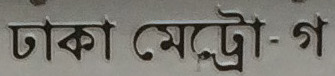
\includegraphics[scale=0.8]{./img/up}
    \caption{upper portion of license plate}
	\label{fig:UP}
    
    
\includegraphics[scale=0.8]{./img/down}
    \caption{bottom part of license plate}
	\label{fig:DOWN}
    
    \end{figure} 
\subsection{Plate fonts}
Digital license plate is offering verified fonts, but in Bangladesh those rules are not strictly followed by all vehicle owners. Also the current dataset doesn't have any universal font. So, the fonts can be different but easily understandable for this thesis work.
